\documentclass{beamer}

\usepackage[utf8]{inputenc}
%\usepackage{default}

\begin{document}

\begin{frame}
 \frametitle{ProteinPrediction II}
 PPII Ex6 - Week 6\\
 \hfill \\
 Jonathan Boidol, Rene Schoeffel, Yann Sp\"ori
\end{frame}

\begin{frame}
  \frametitle{Confidence score}
 	\begin{itemize}
 		\item prediction from neural net: two output nodes 
 		\item difference of prediction as confidence
 		\item (normalize in [0;1])
 	\end{itemize}

\end{frame}

\begin{frame}
	\frametitle{F-measure}
	\begin{minipage}{0.45\textwidth}
	First try: 4 Features
	\begin{itemize}
		\item maxEvalue
		\item NoHits
		\item AvgEvalue
		\item longestHitEValue
		\item F-max: 0.0053 $\cdots$
	\end{itemize}
	\end{minipage}
	\begin{minipage}{0.5\textwidth}
		\centering
		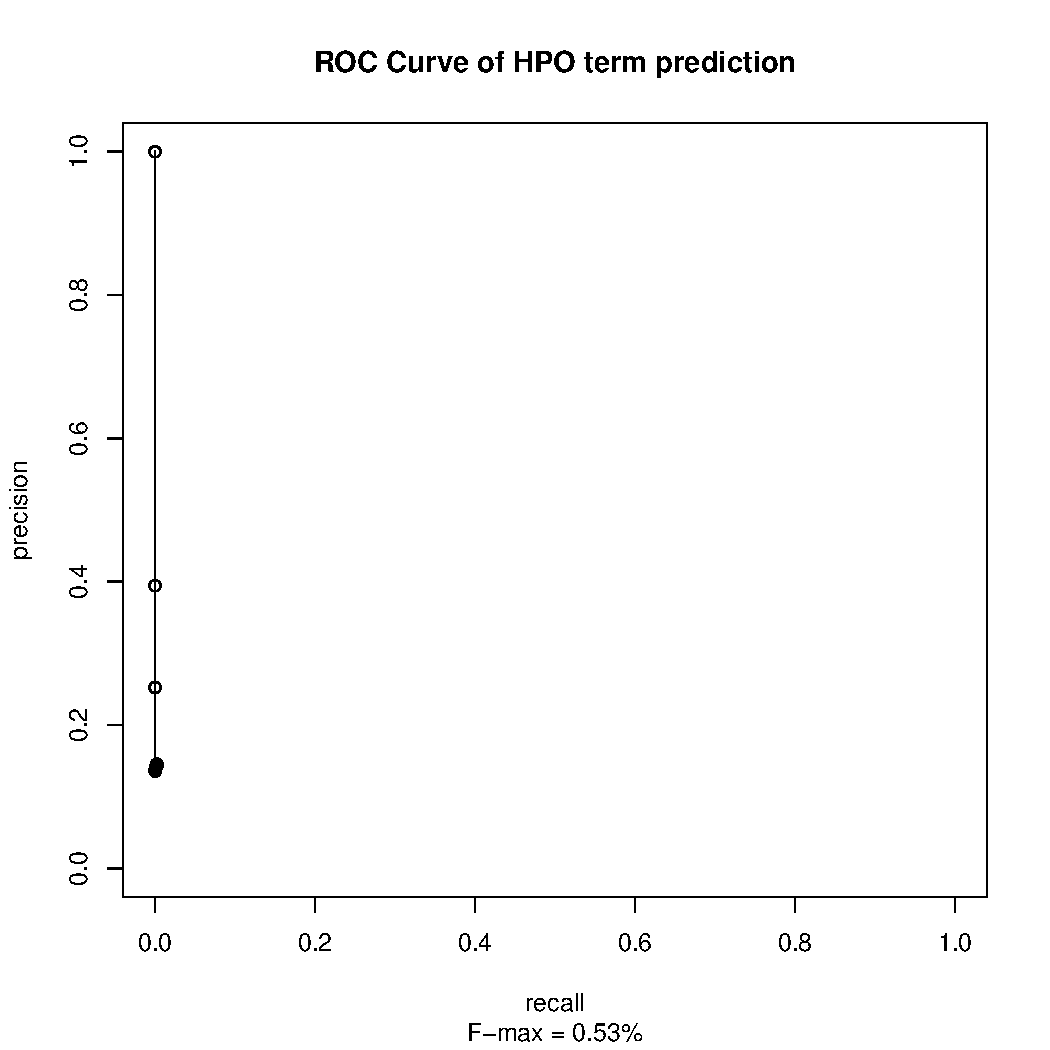
\includegraphics[width=\textwidth]{../../data/ROC_1.pdf}
	
	\end{minipage}

\end{frame}
	
\begin{frame}
\frametitle{F-measure}
\begin{minipage}{0.45\textwidth}
	Next try: 2 more Features
	\begin{itemize}
		\item longestHitLength
		\item AvgHitLength
		\item F-max: 0.1315
		\item will hopefully be improved
		\end{itemize}
	\end{minipage}
	\begin{minipage}{0.5\textwidth}
		\centering	
		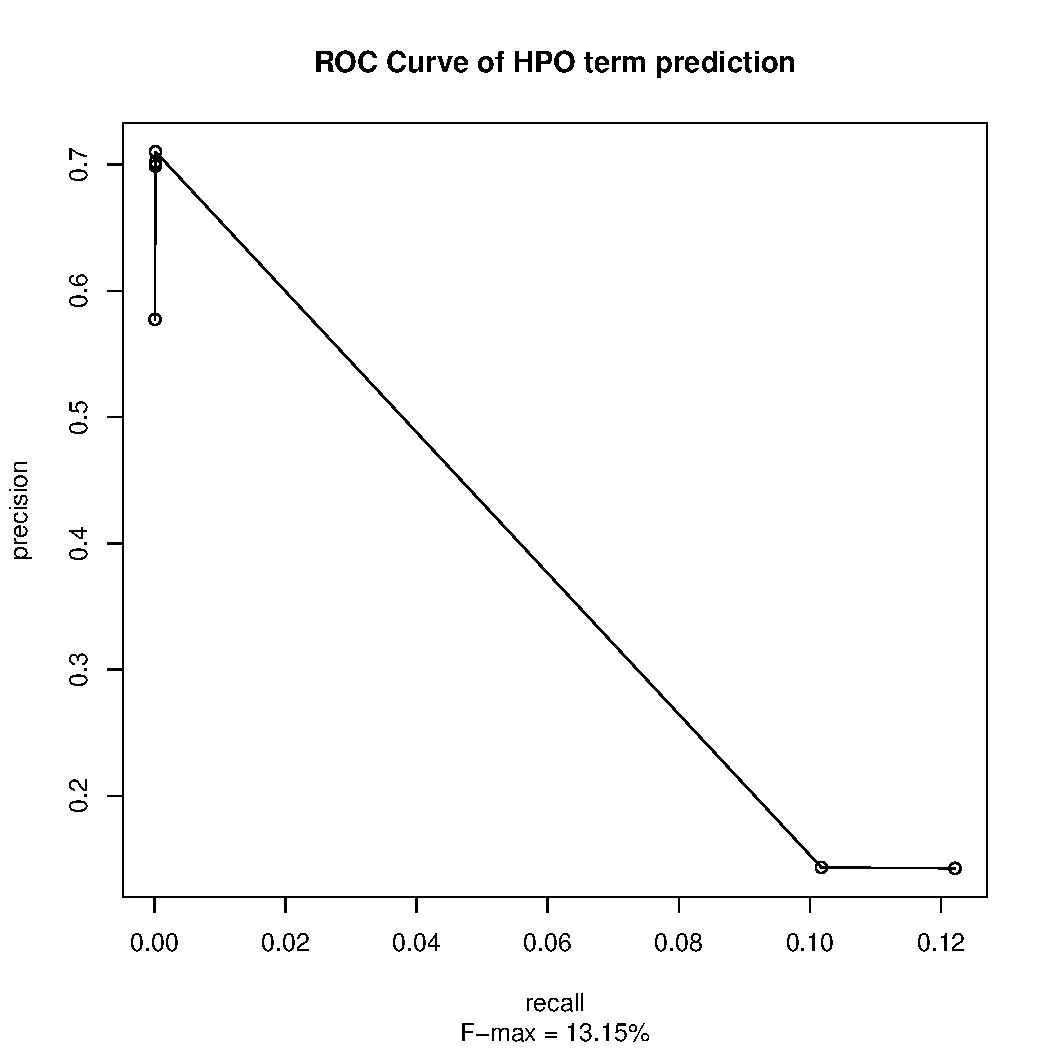
\includegraphics[width=\textwidth]{../../data/ROC_2.pdf}
	\end{minipage}
\end{frame}

\end{document}
